\section{Auswertung}
\label{sec:Auswertung}
\subsection{Untersuchung der Gitterstruktur von HOPG}
Zur Untersuchung der Gitterstruktur werden zwei Scandurchgänge verwendet mit jeweils einem vorwärts und einem rückwärts Scan. Diese sind in Abbildung \ref{fig:Gitter_Graphit_1} und \ref{fig:Gitter_Graphit_2} zu sehen. Zur Bestimmung des Übernächsten-Nachbarn-Abstands $d$ werden die Längen der beiden Gittervektoren $\vec{g}_1$ und $\vec{g}_2$ gemessen. Dies erfolgt graphisch über mehrere Einheitszellen hinweg. Der Mittelwert beider Längen der Gittervektoren entspricht $d$. $\vec{g}_1$ wird aus den annähernd vertikalen Linien bestimmt und $\vec{g}_2$ aus den diagonalen Linien. 
\begin{figure}[h]
    \centering
    \begin{subfigure}{.475\linewidth}
        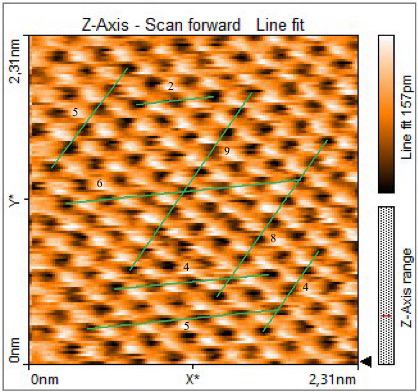
\includegraphics[width=\linewidth]{Messdaten/Gitter_Graphit/1_Bild_forward.png}
    \end{subfigure}\hfill 
    \begin{subfigure}{.475\linewidth}
        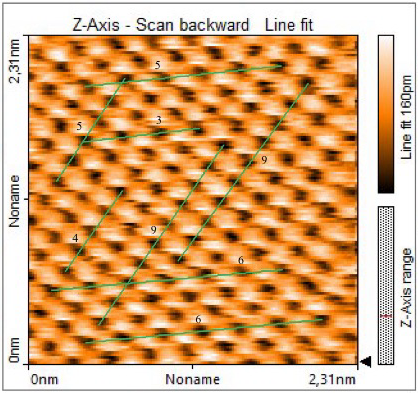
\includegraphics[width=\linewidth]{Messdaten/Gitter_Graphit/1_Bild_backwards.png}
    \end{subfigure}
    \caption{Erster Scan der Gitterstruktur von HOPG mit graphischer Auswertung.}
    \label{fig:Gitter_Graphit_1}
\end{figure}
Die graphisch ermittelten Längen der aus den Gittervektoren sind in Tabelle \ref{tab:Graphit_Bild_1} und \ref{tab:Graphit_Bild_2} aufgeführt. 

\begin{table}[h]
    \centering
    \caption{Graphisch ermittelte Länge der Gittervektoren des ersten Graphitscans.}
    \label{tab:Graphit_Bild_1}
    \begin{tblr}{colspec= c c c c}
        \toprule
        $\left|\vec{g}_{\text{1,vor}} \right| / \unit{\pico\meter}$ & $\left|\vec{g}_{\text{2,vor}} \right| / \unit{\pico\meter}$ & $\left|\vec{g}_{\text{1,rück}} \right| / \unit{\pico\meter}$ & $\left|\vec{g}_{\text{2,rück}}\right| / \unit{\pico\meter}$ \\
        \midrule
        $276,1  \pm 12,8$   & $175,1  \pm  5,1$    &  $277,6   \pm  5,1$   & $173,2    \pm 5,1$ \\
        $278,0  \pm 4,3 $   & $169,6  \pm  2,8$    &  $272,4   \pm  8,5$   & $171,5    \pm 6,4$ \\
        $274,1  \pm 6,4 $   & $169,3  \pm  3,2$    &  $273,3   \pm  4,3$   & $170,8    \pm 2,8$ \\
        $274,0  \pm 5,1 $   & $173,3  \pm  6,4$    &  $278,0   \pm  4,3$   & $171,5    \pm 2,8$ \\
        \bottomrule
    \end{tblr}
\end{table}



\begin{figure}[h]
    \centering
    \begin{subfigure}{.475\linewidth}
      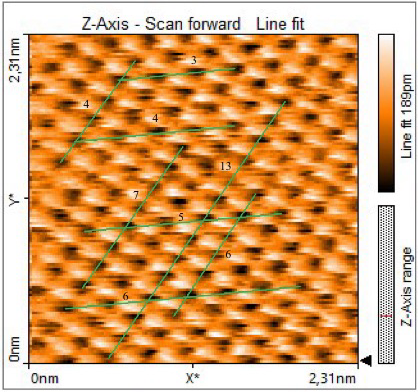
\includegraphics[width=\linewidth]{Messdaten/Gitter_Graphit/2_Bild_forwards.png}
    \end{subfigure}\hfill 
    \begin{subfigure}{.475\linewidth}
      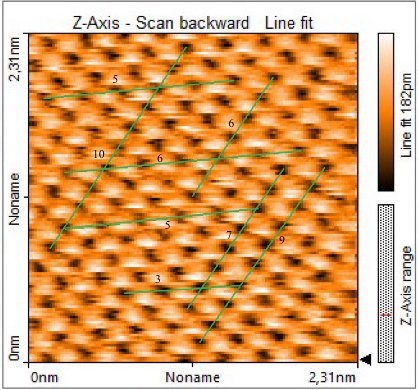
\includegraphics[width=\linewidth]{Messdaten/Gitter_Graphit/2_Bild_backwards.png}
    \end{subfigure}
    \caption{Zweiter Scan der Gitterstruktur von HOPG mit graphischer Auswertung.}
    \label{fig:Gitter_Graphit_2}
\end{figure}

\begin{table}[h]
  \centering
  \caption{Graphisch ermittelte Länge der Gittervektoren des zweiten Graphitscans.}
  \label{tab:Graphit_Bild_2}
  \begin{tblr}{colspec= c c c c}
      \toprule
      $\left|\vec{g}_{\text{1,vor}} \right| / \unit{\pico\meter}$ & $\left|\vec{g}_{\text{2,vor}} \right| / \unit{\pico\meter}$ & $\left|\vec{g}_{\text{1,rück}} \right| / \unit{\pico\meter}$ & $\left|\vec{g}_{\text{2,rück}}\right| / \unit{\pico\meter}$ \\
      \midrule
       $267,6    \pm  8,5$   & $177,9  \pm 5,1$   &   $270,1  \pm 5,1$ & $172,9  \pm  2,6$  \\  
       $283,3    \pm  6,4$   & $174,6  \pm 3,6$   &   $276,4  \pm 4,3$ & $167,7  \pm  4,3$  \\ 
       $277,3    \pm  5,1$   & $168,7  \pm 2,0$   &   $274,0  \pm 5,1$ & $170,6  \pm  3,6$  \\ 
       $276,4    \pm  4,3$   & $172,3  \pm 4,3$   &   $274,3  \pm 8,5$ & $167,5  \pm  2,8$  \\ 
      \bottomrule
  \end{tblr}
\end{table}

Die durchschnittliche Länge der Gittervektoren ist 
%Horizontale_Laengen_Durchschnitt:  0.2752+/-0.0016
%Vertikale_Laengen_Durchschnitt:  0.1716+/-0.0010
$ \left|\vec{g}_{\text{1}} \right| = (275,2 \pm 1,6) \,  \unit{\pico\meter} \,\, \text{und} \,\, \left|\vec{g}_{\text{2}} \right| = (171,6 \pm 1,0) \, \unit{\pico\meter} \, .$
Daraus ergibt sich $ d = (223,4 \pm 1,0)  \, \unit{\pico\meter} \, .$
Der Winkel zwischen den Gittervektoren ergibt sich durch die Berechnung mithilfe von 
\begin{equation*}
  \alpha = \arccos{\left(\frac{\vec{g}_{\text{1}} \cdot \vec{g}_{\text{2}}}{\left|\vec{g}_{\text{1}} \right| \left|\vec{g}_{\text{2}} \right|}\right)}
\end{equation*}
 zu $\alpha = (49,37 \pm 0,39)°$.
\floatbarrier

\subsection{Untersuchung der Oberfläche von Gold}
Zur Untersuchung der Stufen auf einer Goldoberfläche werden die Bilder, die in \autoref{fig:Gold} zu sehen sind, verwendet. Der Scan \ref{fig:fremdes} wurde nicht während der Durchführung selbst aufgenommen, sondern von einer anderen Versuchsdurchführung für die Auswertung zur Verfügung gestellt. Der Scan \ref{fig:eigenes} wurde selbstsändig aufgezeichnet. Aus beiden Scans werden vier verschiedene Höhenprofile mithilfe der Software Gwyddith extrahiert und für die Auswertung verwendet. Die ausgewählten Höhenprofile sind in \autoref{fig:Hoehenprofil_Bild_1} und \autoref{fig:Hoehenprofil_Bild_2} dargestellt. Die daraus ausgewählten Höhenunterschiede $\Delta z$ sind in \autoref{tab:Hoehendiff} aufgelistet und in \autoref{fig:Hoehendiff} dargestellt.
In \autoref{fig:Hoehendiff} ist bei beiden Scans eine Lücke zwischen zwei Häufungen zu sehen. Aus den Häufungspunkten wird die Dicke einer Atomschicht bestimmt. Der Mittelwert der Höhe der einatomigen Stufe des erstens Scans ist $\Delta z_{\text{eigen}} = (0,249 \pm 0,029) \,  \unit{\nano\meter}$ und des zweiten Scans ist $\Delta z_{\text{nicht eigen}} = (0,269 \pm 0,030)\,  \unit{\nano\meter}$. Die aus beiden gemittelte Höhe beträgt $\Delta z_{\text{beide}} = (0,259 \pm 0,021)\,  \unit{\nano\meter}$.

%Oberere_Haufungspunkt_eigen_Mittelwert:  0.8380000000000001 0.023288051299611427
%Unterer_Haufungspunkt_eigen_Mittelwert:  0.5894 0.01747455292704222
%Unterschied_eigener_Haufungspunkt:  0.249+/-0.029
%Oberere_Haufungspunkt_anderes_Mittelwert:  0.47941666666666666 0.024024753123107482
%Unterer_Haufungspunkt_anderes_Mittelwert:  0.2104285714285714 0.018453102904463548
%Unterschied_anderer_Haufungspunkt:  0.269+/-0.030
%Beide zusammen : 0.259+/-0.021

\begin{figure}[]
  \centering
  \subfloat[Scan einer Goldoberfläche.]{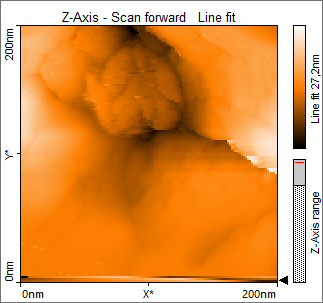
\includegraphics[width=0.4\textwidth]{Messdaten/Goldfotos/Einzeldings(1).PNG}\label{fig:fremdes}}
  \hfill
  \subfloat[Eigener aufgenommener Scan einer Goldoberfläche.]{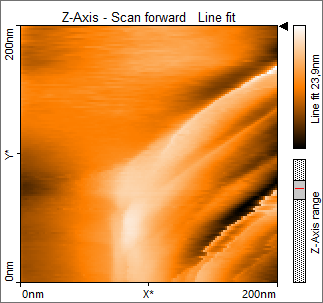
\includegraphics[width=0.4\textwidth]{Messdaten/Goldfotos/Unser_Gold_Einzeldings.PNG}\label{fig:eigenes}}
  \caption{Aufgenomme Scans von Goldoberflächen, die zur Erstellung der Höhenprofile verwendet werden.}
  \label{fig:Gold}
\end{figure}


\begin{figure}[]
    \centering
    \begin{subfigure}{.475\linewidth}
        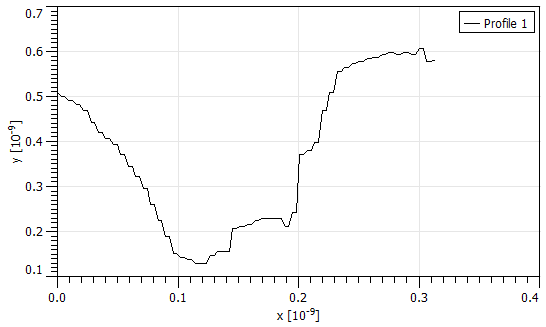
\includegraphics[width=\linewidth]{Messdaten/Hoehenprofil_anderes/1.png}
      \end{subfigure}\hfill 
      \begin{subfigure}{.475\linewidth}
        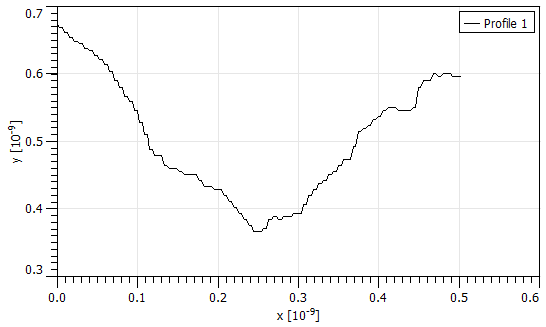
\includegraphics[width=\linewidth]{Messdaten/Hoehenprofil_anderes/2.png}
      \end{subfigure}
      \medskip 

      \begin{subfigure}{.475\linewidth}
        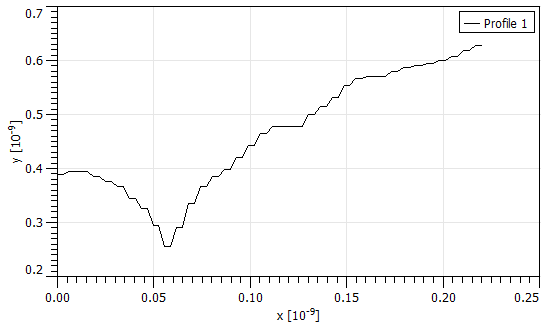
\includegraphics[width=\linewidth]{Messdaten/Hoehenprofil_anderes/3.png}
      \end{subfigure}\hfill 
      \begin{subfigure}{.475\linewidth}
        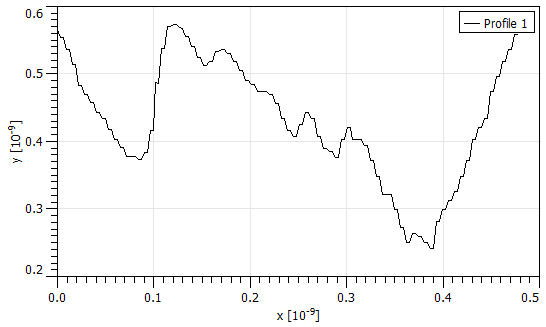
\includegraphics[width=\linewidth]{Messdaten/Hoehenprofil_anderes/4.png}
      \end{subfigure}\hfill 
      \caption{Höhenprofile des 1. Scans an ausgewählten Stellen.}
      \label{fig:Hoehenprofil_Bild_1}
  \end{figure}

\begin{figure}[]
    \centering
    \begin{subfigure}{.475\linewidth}
        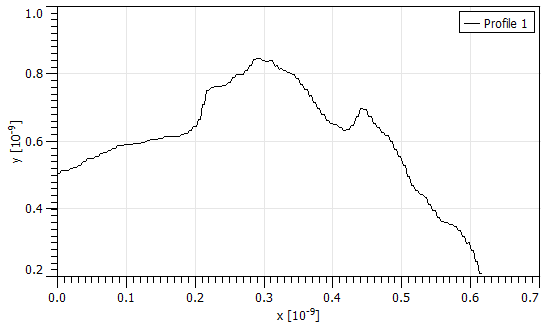
\includegraphics[width=\linewidth]{Messdaten/Hoehenprofile_unseres/1.png}
    \end{subfigure}\hfill 
    \begin{subfigure}{.475\linewidth}
        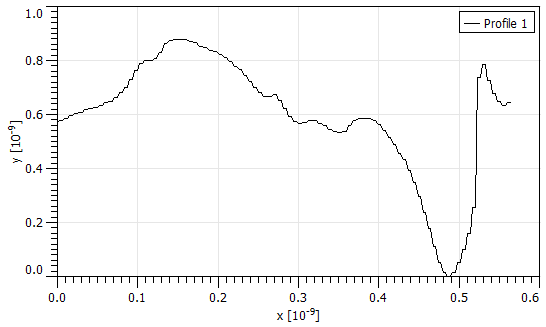
\includegraphics[width=\linewidth]{Messdaten/Hoehenprofile_unseres/2.png}
    \end{subfigure}
    \medskip 

    \begin{subfigure}{.475\linewidth}
        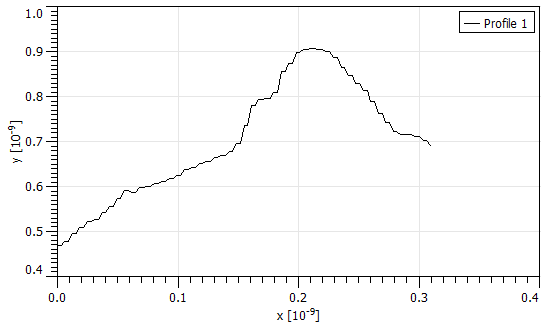
\includegraphics[width=\linewidth]{Messdaten/Hoehenprofile_unseres/3.png}
    \end{subfigure}\hfill 
    \begin{subfigure}{.475\linewidth}
        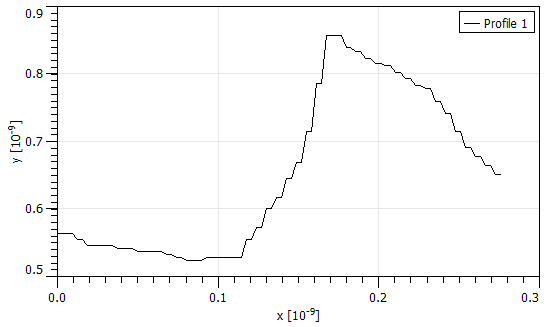
\includegraphics[width=\linewidth]{Messdaten/Hoehenprofile_unseres/4.png}
    \end{subfigure}\hfill 
    \caption{Höhenprofile des 2. Scans an ausgewählten Stellen.}
    \label{fig:Hoehenprofil_Bild_2}
\end{figure}

\begin{table}[h]
  \centering
  \caption{Höhendifferenzen $\Delta z$ verschiedener Stufen aus den ausgewählte Höhenprofilen.}
  \label{tab:Hoehendiff}
  \begin{tblr}{colspec= c c c}
      \toprule
      $\Delta z_{\text{eigen}} \, / \unit{\nano\meter}$ & $\Delta z_{\text{nicht eigen}} \, / \unit{\nano\meter}$ & $\Delta z_{\text{nicht eigen}} \, / \unit{\nano\meter}$ \\
      \midrule
       $0,84$ &  $0,61$ &  $0,48$ \\
       $0,76$ &  $0,23$ &  $0,26$ \\
       $0,63$ &  $0,21$ &  $0,57$ \\
       $0,62$ &  $0,16$ &  $0,51$ \\
       $0,88$ &  $0,13$ &  $0,41$ \\
       $0,78$ &  $0,55$ &  $0,38$ \\
       $0,58$ &  $0,47$ &  $0,25$ \\
       $0,91$ &  $0,45$ &  $0,24$ \\
       $0,59$ &  $0,39$ &         \\
       $0,86$ &  $0,37$ &         \\
       $0,53$ &  $0,57$ &         \\    
      \bottomrule
  \end{tblr}
\end{table}

\begin{figure}[]
  \centering
  \includegraphics[width=0.7\linewidth]{build/plot.pdf}
  \caption{Darstellung der Höhendifferenzen beider Scans.}
  \label{fig:Hoehendiff}
\end{figure}

% \begin{figure}
%   \centering
%   \includegraphics{plot.pdf}
%   \caption{Plot.}
%   \label{fig:plot}
% \end{figure}

%Siehe \autoref{fig:plot}!